\documentclass[dvipdfmx]{beamer}
\usetheme[secheader]{Boadilla}
% \usepackage{beamerthemesplit} // Activate for custom appearanced
%\setbeamertemplate{caption}[numbered]
\usefonttheme[onlymath]{serif} %数式をゴシックにしない
\setbeamertemplate{blocks}[rounded] % Blockの影を消す
\useinnertheme{circles} % 箇条書きをシンプルに
\setbeamertemplate{navigation symbols}{} % ナビゲーションシンボルを消す
\setbeamertemplate{footline}[frame number] % フッターはスライド番号のみ
\setbeamercolor{page number in head/foot}{fg=black}
% \usepackage{beamerthemesplit} // Activate for custom appearance
\setlength{\parindent}{1em}  %段落字下げ
\renewcommand{\figurename}{Fig}
\renewcommand{\tablename}{Tab}
\usepackage{tikz}  
\usetikzlibrary{decorations.pathreplacing,calligraphy}
\setbeamerfont{itemize/enumerate subbody}{size=\normalsize}
%\setbeamertemplate{itemize subitem}{\normalsize\raise1.25pt\hbox{\donotcoloroutermaths$\blacktriangleright$}}  %to set the symbol size
\usetikzlibrary{shapes,positioning}
\usepackage{xcolor}
\def\mathunderline#1#2{\color{#1}\underline{{\color{black}#2}}\color{black}}

%def symbol
\newcommand{\normal}{\mathcal{N}}
\newcommand{\exponential}{\mathcal{E}}
\newcommand{\truncnorm}{\mathcal{TN}}
\newcommand{\gam}{\mathcal{G}}
\newcommand{\C}{C}
\newcommand{\one}{1\!\!1}

\title{テンソル同時分解の拡張による\\オミクスデータの統合}
\date{2023年6月3日}
\author {阿部興\footnote{東京医科歯科大学難治疾患研究所} ・島村徹平\footnote{名古屋大学医学系研究科・東京医科歯科大学難治疾患研究所}}

\begin{document}
\frame{
\titlepage
}

\renewcommand*{\thefootnote}{\fnsymbol{footnote}}
\setcounter{footnote}{0} 

\section{背景}
\frame{
\frametitle{動機:分析対象}
\begin{figure}
 \begin{tikzpicture}
\node[draw, rounded corners, fill=gray!10](dna) at (0,0){
\includegraphics[width=.05\textwidth]{img/dna.png}DNA};
\node[draw, rounded corners, fill=gray!10, right = of dna, xshift = +15pt](rna){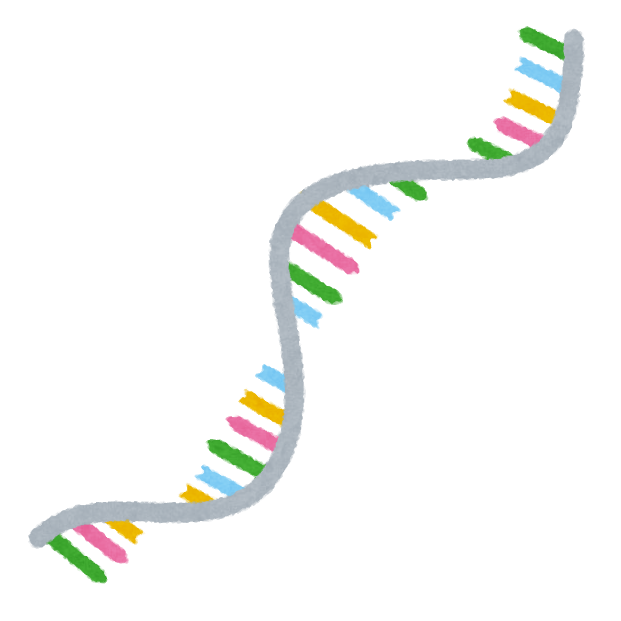
\includegraphics[width=.05\textwidth]{img/body_rna.png}RNA};
\node[draw, rounded corners, fill=gray!10, right = of rna, xshift = +15pt](protein){
\includegraphics[width=.05\textwidth]{img/kagaku_bunshi.png}protein};
\node[draw, rounded corners, fill=gray!10, right = of protein](phenotype) {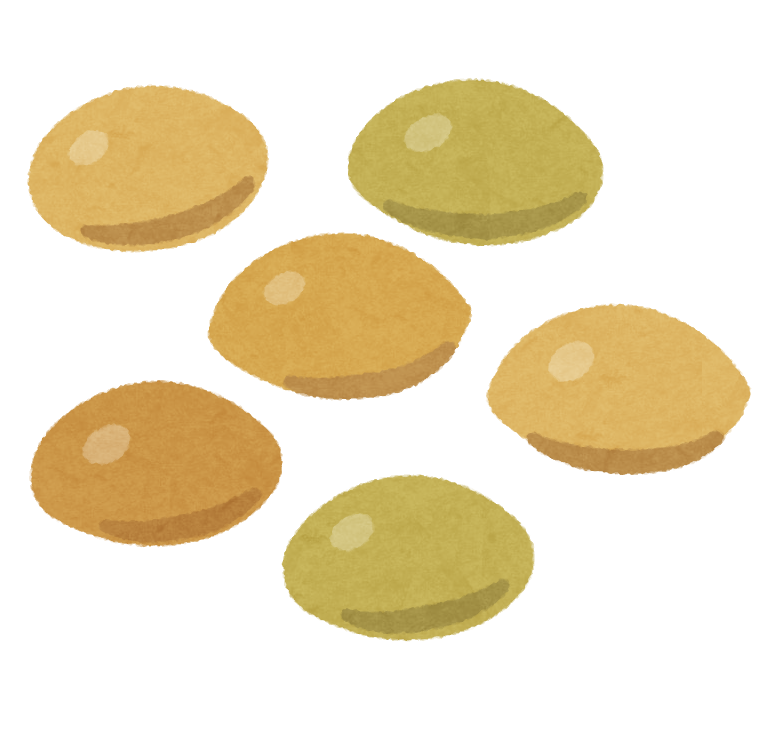
\includegraphics[width=.05\textwidth]{img/nut_renzumame.png}phenotype};
%path
\path[draw, ->, olive](dna)--(rna) node[midway, below, yshift = -2pt]{転写};
\path[draw, ->, olive](rna)--(protein) node[midway, below, yshift = -2pt]{翻訳};
\path[draw, dashed, ->, olive](protein)--(phenotype);
%omics
\node[below= of dna](genomics){genomics};
\node[below= of rna](transcriptomics){transcriptomics};
\node[below= of protein](proteomics){proteomics};

\node[above= of dna, yshift=-5ex]{\textcolor{gray}{モダリティ}};

\path[draw, teal](dna)--(genomics);
\path[draw, teal](rna)--(transcriptomics);
\path[draw, teal](proteomics)--(protein);

\path[draw, teal, dashed](genomics.north west)--(proteomics.north east);
\path[draw, teal, dashed](genomics.south west)--(proteomics.south east);
\path[draw, teal, dashed](genomics.north west)--(genomics.south west);
\path[draw, teal, dashed](proteomics.north east)--(proteomics.east)node[right](omics){-omics};
\end{tikzpicture}
\end{figure}
\begin{itemize}
\item オミクス(omics)データを統合して分析したい
\begin{itemize}
\item[] \structure{積極的理由:}データを補い合い普遍的な特徴を抽出
\item[] \structure{消極的理由:}対応のあるサンプルなので非独立
\end{itemize}
\item 難しさ
\begin{itemize}
\item semi-paired なデータが多い
\item モダリティごとに分布が変わる
\end{itemize}
\end{itemize}
}
\frame{
\frametitle{動機:分析手法}
\begin{figure}
\begin{tabular}{c}
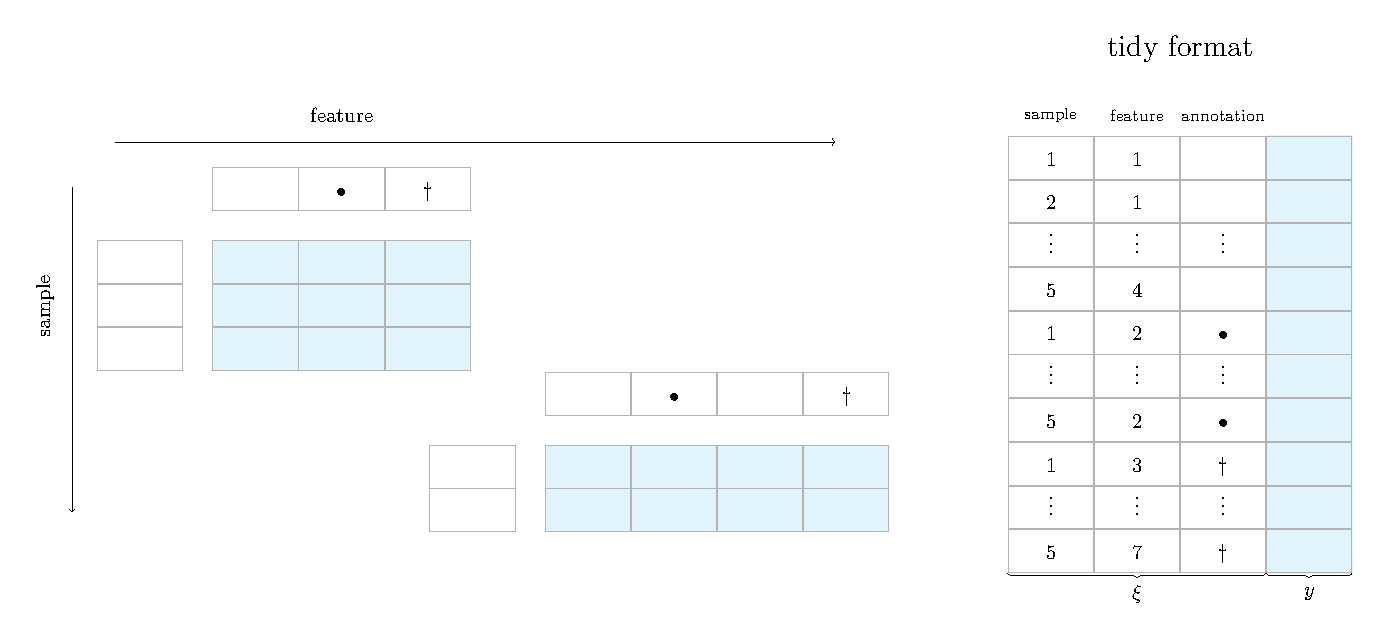
\includegraphics[height=0.4\textheight]{img/mosaic_an} \\
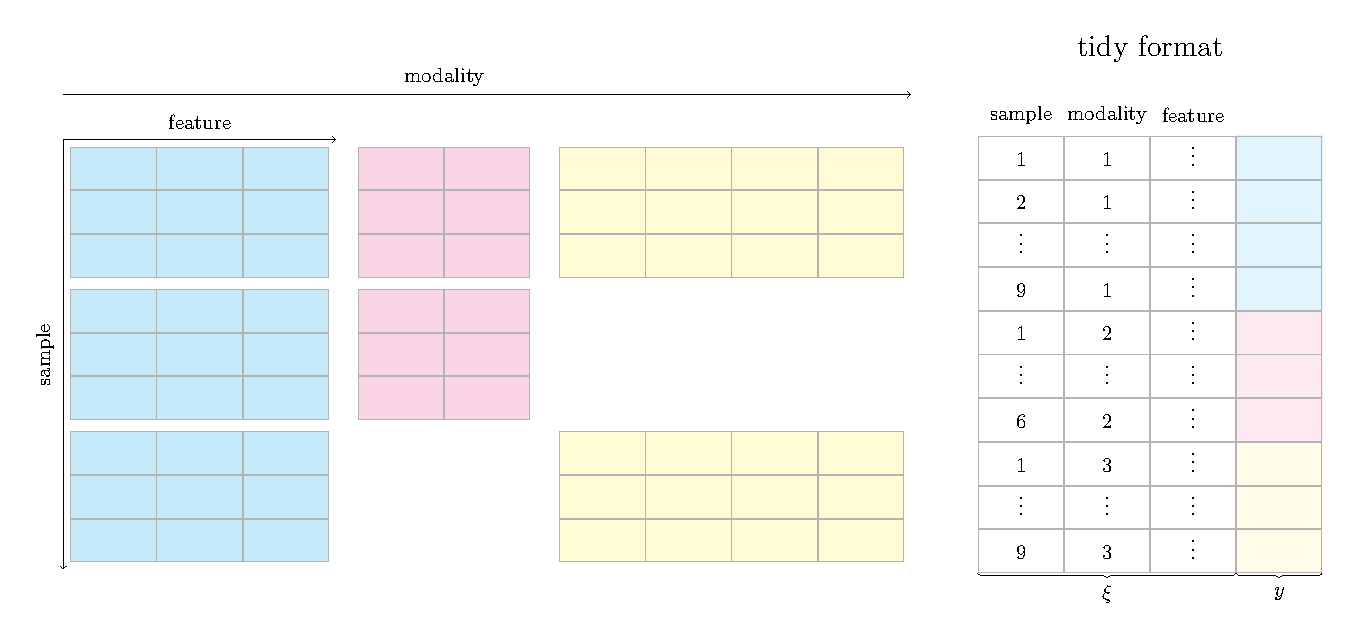
\includegraphics[height=0.4\textheight]{img/mosaic_mm} \\
 tidy-format の利便性をそのままに行列分解ができないか?
\end{tabular}
\end{figure}
}
\frame{
\frametitle{3階のテンソルの場合}
Data:
$$
 Y=(y_{ijk}), \quad y=(y_n) = \operatorname{vec}(Y)
$$

CP分解:
\begin{equation*}
y_{ijk} \approx \sum_{l}v_{il}^{(1)} v_{jl}^{(2)} v_{kl}^{(3)}. 
\end{equation*}

提案法:
\begin{equation}
y_{n} \approx \sum_{l}\prod_{d=1}^D v_{dl}^{x_{nd}} \label{eq_approx}
\end{equation}
ここで, 
\begin{align*}
V=(v_{dl})=\begin{pmatrix}
v^{(1)}\\
v^{(2)}\\
v^{(3)}
\end{pmatrix}
\end{align*}
}
\frame{
\frametitle{内積としての解釈}
\begin{align*}
\sum_{l=1}^L \prod_{d=1}^D v_{dl}^{x_{nd}} &= v_{11}^{x_{n1}} v_{21}^{x_{n2}}\cdots  v_{D1}^{x_{nD}}+ \cdots + v_{1L}^{x_{n1}} v_{2L}^{x_{n2}}\cdots  v_{DL}^{x_{nD}}\\
&=
 \underbrace{
\begin{pmatrix}
v_{d1}^{x_{nd}} &  \ldots  & v_{dL}^{x_{nd}}
 \end{pmatrix} 
 \cdot
 \begin{pmatrix}
\prod _{d' \neq d}v_{d'1}^{x_{nd'}}\\
 \vdots \\
 \prod _{d' \neq d}v_{d'L}^{x_{nd'}}
 \end{pmatrix}
 }_{\mbox{inner product}}
\end{align*}

}
\frame{
\frametitle{アンサンブルとしての解釈}
\begin{align*}
&\sum_{l=1}^L\prod_{d=1}^D v_{dl}^{x_{nd}} \\
&=\frac{1}{L}\sum_{l=1}^L   L \underbrace{\exp\left( \sum_{d=1}^D x_{nd}  \cdot \log v_{dl}\right) }_{\mbox{let $f_{nl}$}}\\
&= \frac{1}{L}\sum_{l=1}^L L f_{nl} \quad \mbox{\structure{(mean of the log-linear predictor)}}
\end{align*}
}
\frame{
\frametitle{モデル(準備)}

式1($y_{n} \approx \sum_{l} \prod_{d=1}^D v_{dl}^{x_{nd}}$)より
\begin{align}
y_n \mid V, \lambda & \sim \normal\left(y_n \mid \sum_{l=1}^L \prod_{d=1}^D v_{dl}^{x_{nd}}, \lambda^{-1}\right) \label{eq_mod1}\\
v_{dl} & \sim \normal(v_{dl} | 0,\tau^{-1}) \label{eq_prior1}\\
\lambda & \sim \gam(\lambda | a,b) \nonumber
\end{align}

\begin{itemize}
\item さらに修正・拡張
\begin{itemize}
\item 解釈性のため:非負制約 
\item マルチオミクスデータの分析のため:分布を変える
\end{itemize}
\end{itemize}
}
\frame{
\frametitle{事前分布:非負制約}
\begin{align*}
v_{dl} & \sim \truncnorm(v_{dl} | 0,\tau^{-1})  \\ \label{eq_prior2}
& \propto \normal(v_{dl} | 0,\tau^{-1})\one_{(0,\infty)}(v_{dl})
\end{align*}
ここで, $\one_{(0,\infty)}(v_{dl})$ は指示関数.
}
\frame{
\frametitle{中間変数}
\begin{itemize}
\item $y_n$ が実数(連続値):
$$
A(x)=x.
$$
\item 
$y_n$ が非負:
$$
A(x)=\begin{cases}x, &x>0\\0 &x\leq 0\end{cases}.
$$
\item
$y_n$ が2値(0 or 1):
$$
A(x)=\one_{(0,\infty)}(x).
$$
\item
$y_n$ が非負の整数:
$$
A(x)=\begin{cases}\lceil x\rceil, & x>0\\0 &x\leq 0\end{cases}.
$$
\end{itemize}
}
\frame{
\frametitle{切断, Rectified, 離散化}
\begin{figure}
\centering
\begin{tabular}{c|cc}
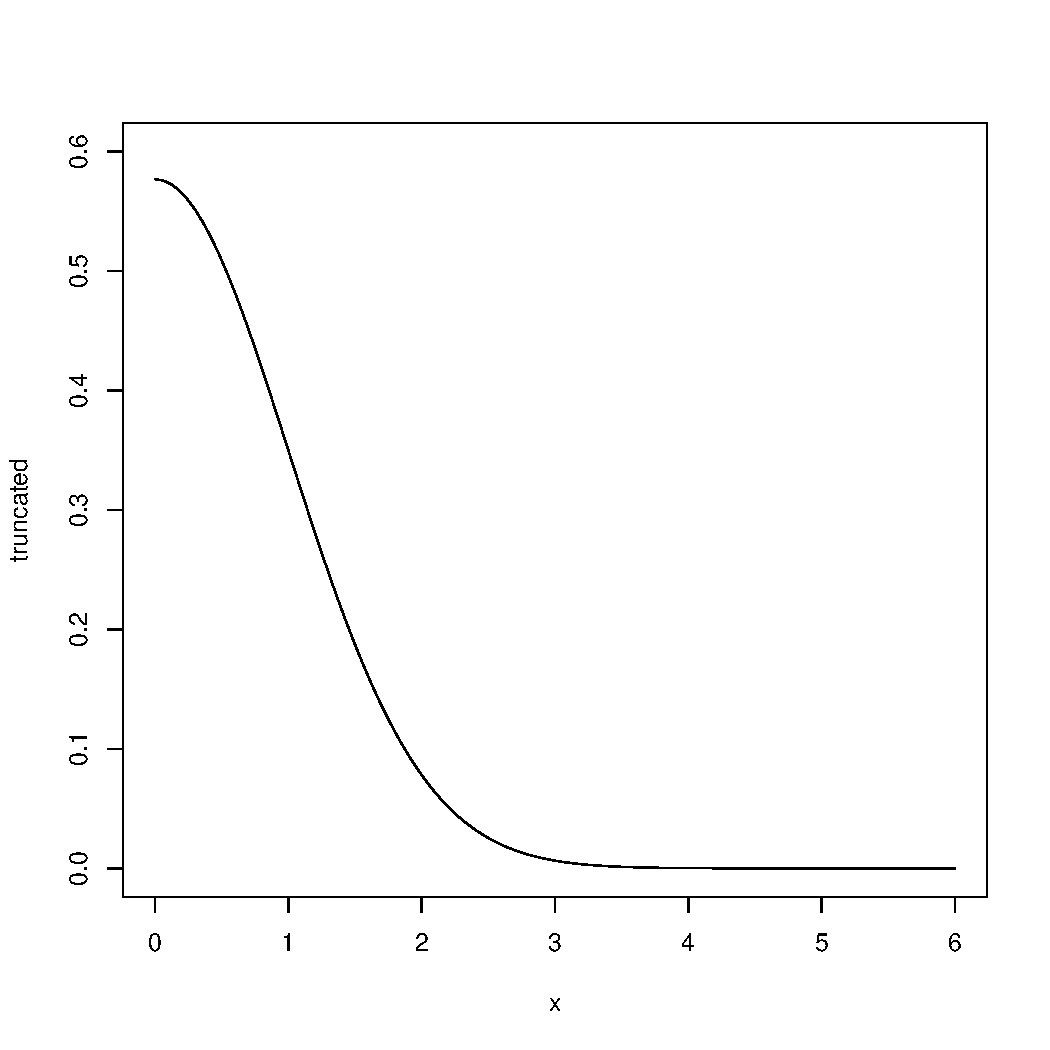
\includegraphics[width=0.3\textwidth]{img/norm_truncated} &
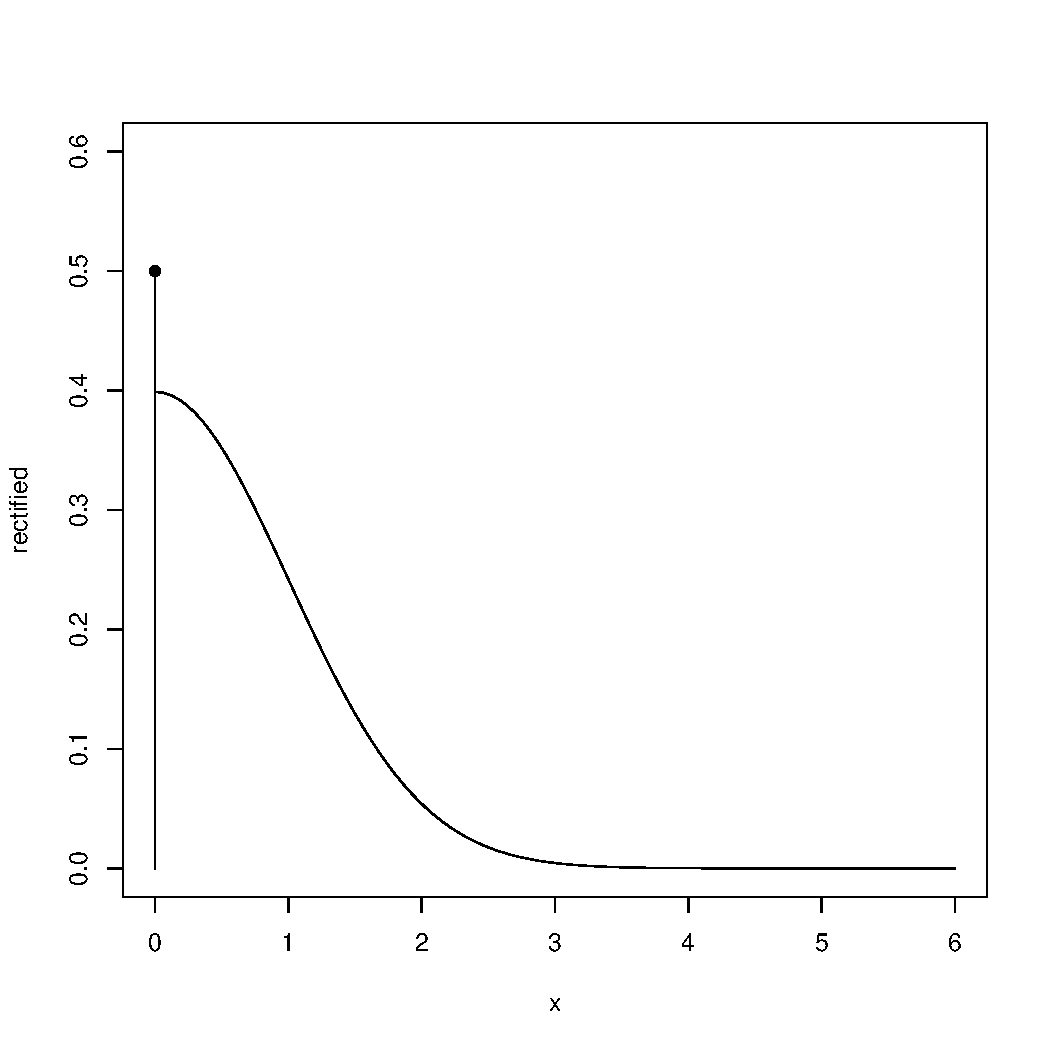
\includegraphics[width=0.3\textwidth]{img/norm_rectified} &
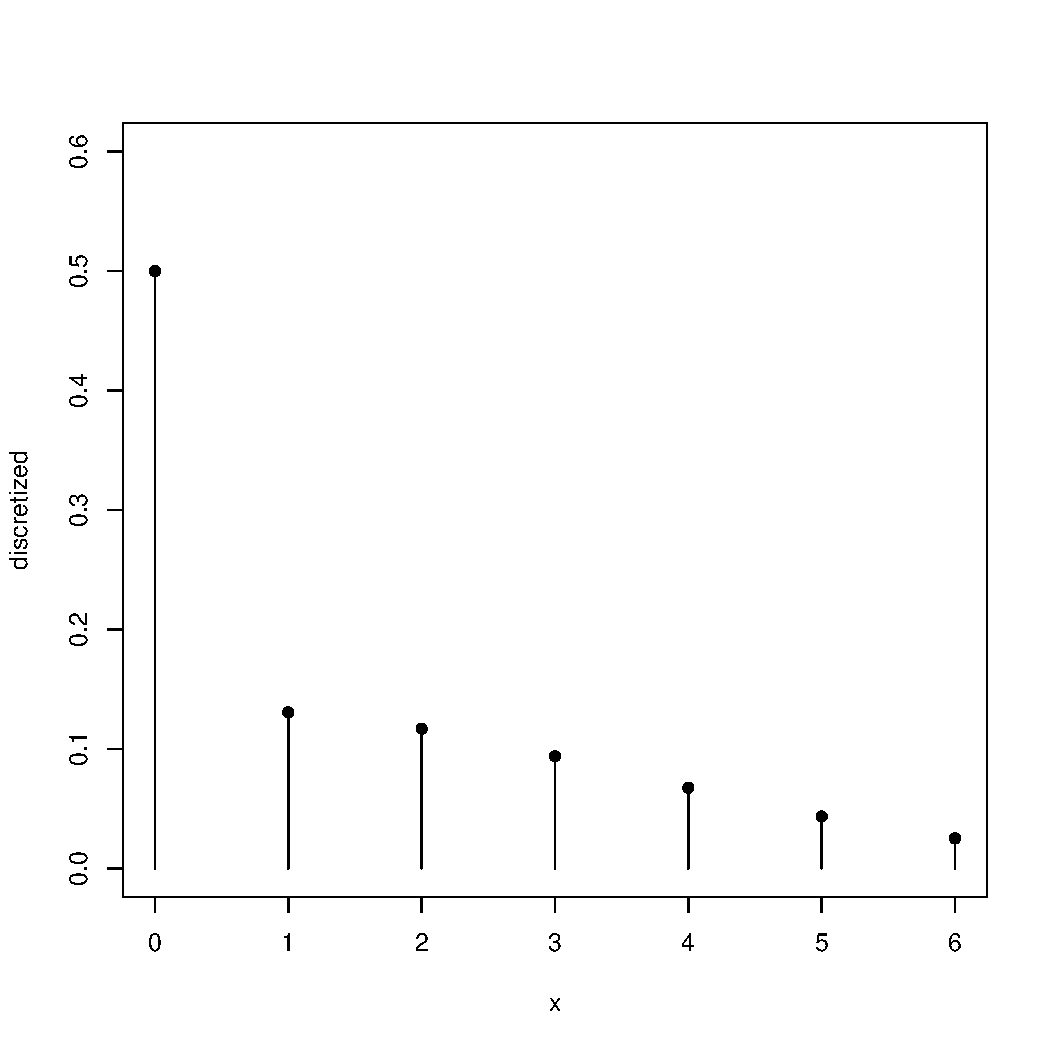
\includegraphics[width=0.3\textwidth]{img/norm_discretized}
\end{tabular}
\caption{左: 潜在変数の事前分布. 右: 観測されるデータのモデル. 一点0で確率を持つ(eg. 重さ, 計数)}
\end{figure}
}
\frame{
\frametitle{モデル}
\begin{equation}
y_{n} = A_{m(n)}(z_{n}), \quad z_{n} \sim \mathcal{N}\left(\sum_{l=1}^L \prod_{d=1}^Dv_{dl}^{x_{nd}}, \lambda^{-1}\right) \label{eq_mod2}    
\end{equation}
ここで $m(n)$ is a function which maps index $n$ to mode $m(n)$. 
}
\frame{
\frametitle{対数尤度}
\begin{align*}
 \ell(v_{dl}) &=\sum_{n=1}^{N} \log p(z|V, X) = \sum_{n=1}^{N}\left(-\frac{\lambda}{2}\left\{ z_n -\sum_{l=1}^L\prod_{d=1}^D v_{dl}^{x_{nd}} \right\}^2\right)+ \C\\
&= -\frac{h_{dl}}{2}\left(v_{dl}^2-2v_{dl}\frac{\eta_{dl}}{h_{dl}}\right) +C,
\end{align*}
ここで,
\begin{align}
\eta_{dl} &= \sum_n x_{nd} \prod_{d' \neq d} v_{dl}^{x_{nd}}\left( z_{n} - \sum_{l'\neq l} \prod_{d' \neq d} v_{dl}^{x_{nd}} \right) \label{eq_eta}\\
h_{dl} &= \sum_n \lambda x_{nd} \prod_{d' \neq d} v_{dl}^{2x_{nd}}. \label{eq_h}
\end{align}
 $C$ は $v_{dl}$ に依存しない定数.
}
\frame{
\frametitle{変分EMアルゴリズム(一般論)}

\begin{itemize}
\item[] データ: $\mathcal{D}=(\mathcal{D}_1,\mathcal{D}_2,\ldots,\mathcal{D}_n)$ 
\item[] $\mathcal{D}$ 全体に影響する \structure{global} な潜在変数: $V$
\item[] $\mathcal{D}_n$ に影響する \structure{local} な潜在変数: $z_n$
\end{itemize}

\begin{align*}
D_{KL}(q\|p) &=\int q(z) \log \frac{q(z)}{p(z_n|\mathcal{D},w)} dz\\
&= E_q [ \log q(z)] - E_q[\log p(z_n|\mathcal{D},w)]
\end{align*}
$q(z) \propto  \exp( E_q[\log p(z_n|\mathcal{D},w)])$ のとき最小.


\begin{block}{変分EMアルゴリズム}
\begin{itemize}
\item []\structure{ E-step:}  $q(z) \propto  \exp( E_q[\log p(z_n|\mathcal{D},w)])$ を更新
\item[] \structure{M-step:}  $q(v_{dl}) \propto  \exp( E_q[\log p(z_n|\mathcal{D},w)])$を更新
\end{itemize}
\end{block}
}
\frame{
\structure{local} な潜在変数 $z_n$ に対しては変分事後分布からサンプリング; 特に $\tilde z_n$ と書く
\begin{itemize}
\item rectified
\begin{align}
q(-z_n) = \begin{cases}
    \mathcal{TN}(-z_n|-f_n, \sigma_n^2) & y_n=0,\\
    z_n = y_n \mbox{~with probability 1} & y_n>0
\end{cases} \label{qz_rect}
\end{align}
\item binary
\begin{align}
q(-z_n) = \begin{cases}
    \mathcal{TN}(-z_n|-f_n, \sigma_n^2) & y_n=0,\\
    \mathcal{TN}(z_n|f_n, \sigma_n^2) & y_n=1
\end{cases} \label{qz_binary}
\end{align}
\item nonnegative integer
\begin{align}
q(-z_n) = \begin{cases}
    \mathcal{TN}(-z_n|-f_n, \sigma_n^2) & y_n=0,\\
    \mathcal{TN}(z_n|f_n, \sigma_n^2) & y_n=1
\end{cases} \label{qz_binary}
\end{align}
\end{itemize}
}
\frame{
\begin{align}
q(v_{dl})= \begin{cases}
\normal(\mu_{dl}, \sigma_{dl}) & \mbox{if the prior of $v_{dl}$ is not truncated} \\
\truncnorm(\mu_{dl}, \sigma_{dl}) & \mbox{if the prior of $v_{dl}$ is truncated},     
\end{cases} \label{qv}
\end{align}
ここで, 
\begin{align*}
\mu_{dl} &=\frac{\langle \eta_{dl} \rangle}{\langle h_{dl}\rangle+\tau/\langle\lambda\rangle},\\
\sigma^2 &=\left(\tau + \langle h_{dl} \rangle \right)^{-1}.
\end{align*}
$\lambda$ の変分事後分布は,  
\begin{align}
    q(\lambda) = \gam\left(N/2 \eta_{dl}, \left(h_{dl}+\tau\right)/2\right). \label{qlam}
\end{align}

}
\frame{
大規模メタアナリシス(学習済みword2vec のように配布), 
因果推論(g-formula), 時空間相関
}
\end{document} 